\chapter{Sistemi di numerazione}
\label{cha:Sistemi di numerazione}
\section{Sistema non posizionale}
\label{sec:sistemanonposizionale}
\mediapriorita{Inserire storia dei sistemi di numerazione}

\section{Sistema posizionale} 
\label{sec:sistemaposizionale}
Un sistema numerico si dice posizionale se le cifre, usate per scrivere un numero, assumono valori diversi modificando la loro posizione.
Un numero è quindi una successione di cifre il cui valore si ottiene moltiplicando la cifra per le potenze di un numero detto base. \[a_1a_2a_3a_4=a_1b^3+a_2b^2+a_3b^1+a_4b^0\] 
\begin{table}
	\centering
	\begin{tabular}{lllll}
	\toprule
	& \multicolumn{4}{c}{\textbf{basi}} \\ 
	\multirow{16}*{\textbf{Cifre}}& \multicolumn{1}{c}{2} & \multicolumn{1}{c}{8} & \multicolumn{1}{c}{10} & \multicolumn{1}{c}{16} \\ 
	\midrule
	& \multicolumn{1}{c}{0} & \multicolumn{1}{c}{0} & \multicolumn{1}{c}{0} & \multicolumn{1}{c}{0} \\ 
	& \multicolumn{1}{c}{1} & \multicolumn{1}{c}{1} & \multicolumn{1}{c}{1} & \multicolumn{1}{c}{1} \\ 
	& \multicolumn{1}{c}{} & \multicolumn{1}{c}{2} & \multicolumn{1}{c}{2} & \multicolumn{1}{c}{2} \\ 
	& \multicolumn{1}{c}{} & \multicolumn{1}{c}{3} & \multicolumn{1}{c}{3} & \multicolumn{1}{c}{3} \\ 
	& \multicolumn{1}{c}{} & \multicolumn{1}{c}{4} & \multicolumn{1}{c}{4} & \multicolumn{1}{c}{4} \\ 
	& \multicolumn{1}{c}{} & \multicolumn{1}{c}{5} & \multicolumn{1}{c}{5} & \multicolumn{1}{c}{5} \\ 
	& \multicolumn{1}{c}{} & \multicolumn{1}{c}{6} & \multicolumn{1}{c}{6} & \multicolumn{1}{c}{6} \\ 
	& \multicolumn{1}{c}{} & \multicolumn{1}{c}{7} & \multicolumn{1}{c}{7} & \multicolumn{1}{c}{7} \\ 
	& \multicolumn{1}{c}{} & \multicolumn{1}{c}{} & \multicolumn{1}{c}{8} & \multicolumn{1}{c}{8} \\ 
	& \multicolumn{1}{c}{} & \multicolumn{1}{c}{} & \multicolumn{1}{c}{9} & \multicolumn{1}{c}{9} \\ 
	& \multicolumn{1}{c}{} & \multicolumn{1}{c}{} & \multicolumn{1}{c}{} & \multicolumn{1}{c}{10} \\ 
	& \multicolumn{1}{c}{} & \multicolumn{1}{c}{} & \multicolumn{1}{c}{} & \multicolumn{1}{c}{A} \\ 
	& \multicolumn{1}{c}{} & \multicolumn{1}{c}{} & \multicolumn{1}{c}{} & \multicolumn{1}{c}{B} \\ 
	& \multicolumn{1}{c}{} & \multicolumn{1}{c}{} & \multicolumn{1}{c}{} & \multicolumn{1}{c}{C} \\ 
	& \multicolumn{1}{c}{} & \multicolumn{1}{c}{} & \multicolumn{1}{c}{} & \multicolumn{1}{c}{D} \\ 
	& \multicolumn{1}{c}{} & \multicolumn{1}{c}{} & \multicolumn{1}{c}{} & \multicolumn{1}{c}{E} \\ 
	& \multicolumn{1}{c}{} & \multicolumn{1}{c}{} & \multicolumn{1}{c}{} & \multicolumn{1}{c}{F} \\ 
	\bottomrule
	\end{tabular}
	\caption{Basi e cifre}
	\label{tab:bassi&cifre}
\end{table}
\section{Cambio di base}
\label{sec:cambiodibase}
\subsection{Da altre basi a base 10}
\subsection{Da base 10 a altre basi}
\begin{tabular}{lllllllll}
\multicolumn{1}{l|}{310} & 2 &  &  &  &  &  &  &  \\ 
\cline{2-2}
\multicolumn{1}{l|}{0} & \multicolumn{1}{l|}{155} & 2 &  &  &  &  &  &  \\ 
\cline{3-3}
& \multicolumn{1}{l|}{1} & \multicolumn{1}{l|}{77} & 2 &  &  &  &  &  \\ 
\cline{4-4}
&  & \multicolumn{1}{l|}{1} & \multicolumn{1}{l|}{38} & 2 &  &  &  &  \\ 
\cline{5-5}
&  &  & \multicolumn{1}{l|}{0} & \multicolumn{1}{l|}{19} & 2 &  &  &  \\ 
\cline{6-6}
&  &  &  & \multicolumn{1}{l|}{1} & \multicolumn{1}{l|}{9} & 2 &  &  \\ 
\cline{7-7}
&  &  &  &  & \multicolumn{1}{l|}{1} & \multicolumn{1}{l|}{4} & 2 &  \\ 
\cline{8-8}
&  &  &  &  &  & \multicolumn{1}{l|}{0} & \multicolumn{1}{l|}{2} & 2 \\ 
\cline{9-9}
&  &  &  &  &  &  & \multicolumn{1}{l|}{0} & 1 \\ 
\end{tabular}
\subsubsection{Operazioni}
\subsection{Base sedici}
\subsubsection{Conversioni}
\subsubsection{Operazioni}
\begin{table}[H]
	\centering
	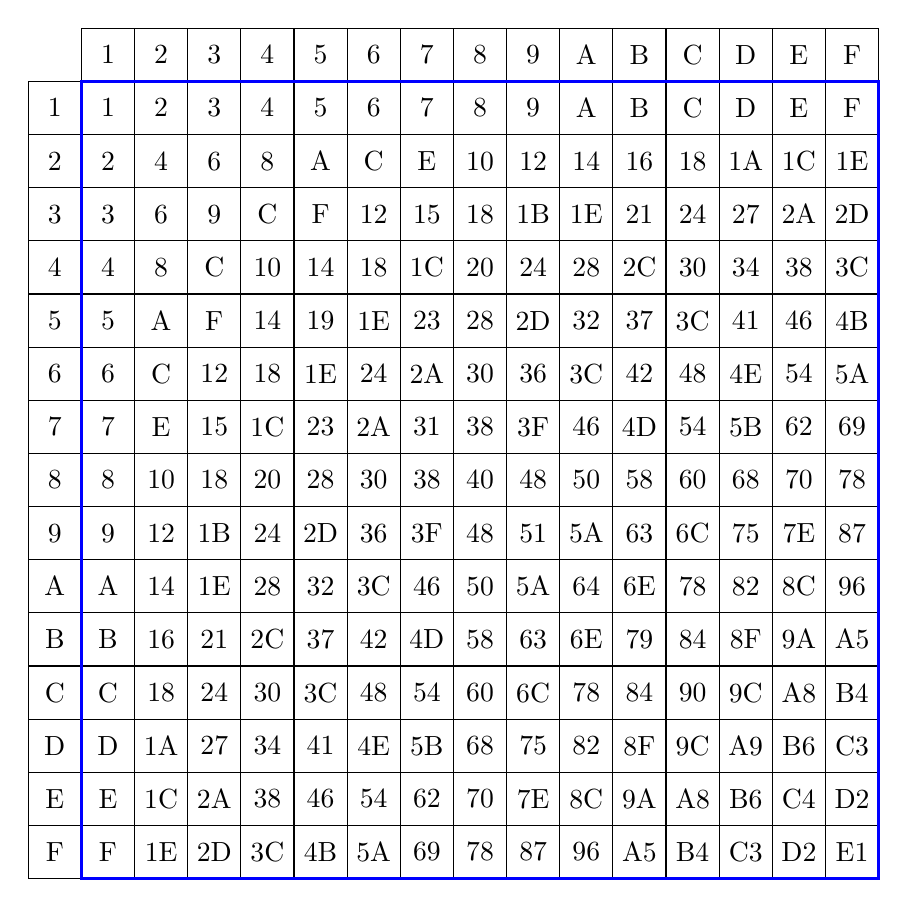
\begin{tikzpicture}[scale=0.675]
		% grid definition
		\draw (-1,0) grid (15,15);
		\draw (0,10) grid (15,16);
		\draw[line width=1pt, color=blue] (0,0) rectangle (15,15);
		
		% fill numbers
		\foreach \x in {1,2,3,...,15}
		\foreach \y in {1,2,3,...,15}
		\draw[shift={(-.5,-.5)}] (\x ,\y) node {\pgfmathHex{\number\numexpr\x*(16-\y)}\pgfmathresult\relax};
		
		% fill first row
		\foreach \x in {1,2,3,...,15}
		\draw[shift={(-.5,-.5)}] (\x , 16) node {\pgfmathHex{\x}\pgfmathresult};
		
		% fill first column
		\foreach \y in {1,2,3,...,15}
		\draw[shift={(-.5,-.5)}] (0, 16-\y) node {\pgfmathHex{\y}\pgfmathresult};
	\end{tikzpicture}
	\caption{Tavola Prodotti esadecimale}
	\label{tab:TavolaPitagoricaesadecimale}
\end{table}
\begin{table}[H]
	\centering
	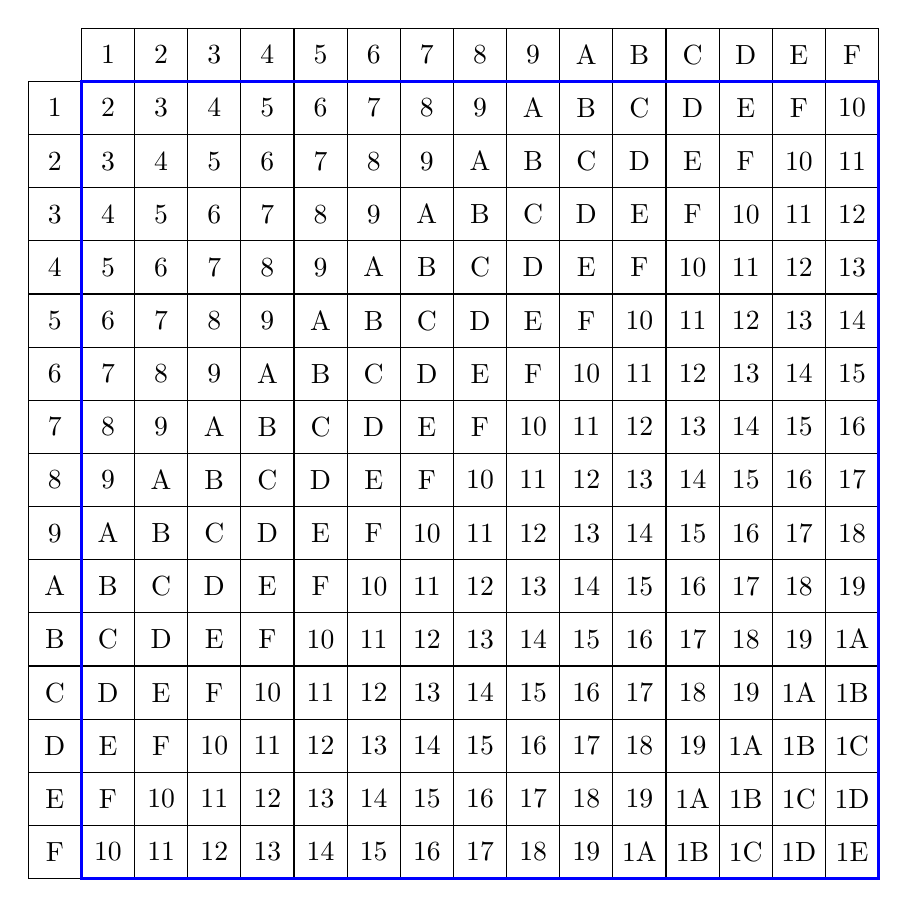
\begin{tikzpicture}[scale=0.675]
		% grid definition
		\draw (-1,0) grid (15,15);
		\draw (0,10) grid (15,16);
		\draw[line width=1pt, color=blue] (0,0) rectangle (15,15);
		
		% fill numbers
		\foreach \x in {1,2,3,...,15}
		\foreach \y in {1,2,3,...,15}
		\draw[shift={(-.5,-.5)}] (\x ,\y) node {\pgfmathHex{\number\numexpr\x+(16-\y)}\pgfmathresult\relax};
		
		% fill first row
		\foreach \x in {1,2,3,...,15}
		\draw[shift={(-.5,-.5)}] (\x , 16) node {\pgfmathHex{\x}\pgfmathresult};
		
		% fill first column
		\foreach \y in {1,2,3,...,15}
		\draw[shift={(-.5,-.5)}] (0, 16-\y) node {\pgfmathHex{\y}\pgfmathresult};
	\end{tikzpicture}
	\caption{Tavola somma esadecimale}
	\label{tab:Tavolaaddizioniesadecimale}
\end{table}
\subsection{Base otto}
\subsubsection{Conversioni}



\begin{table}[H]
	\centering
	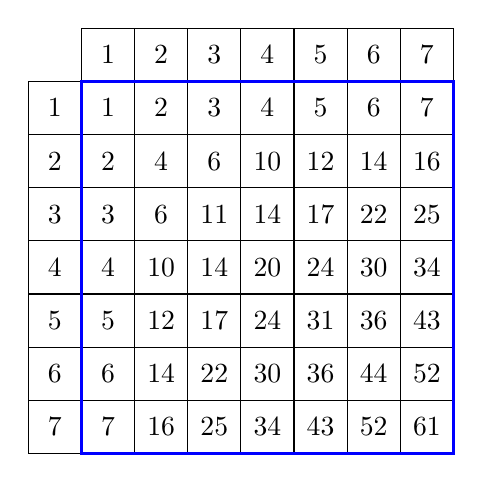
\begin{tikzpicture}[scale=0.675]
		% grid definition
		\draw (-1,0) grid (7,7);
		\draw (0,7) grid (7,8);
		\draw[line width=1pt, color=blue] (0,0) rectangle (7,7);
		
		% fill numbers
		\foreach \x in {1,2,3,...,7}
		\foreach \y in {1,2,3,...,7}
		\draw[shift={(-.5,-.5)}] (\x ,\y) node { \pgfmathoct{\number\numexpr\x*(8-\y)}\pgfmathresult\relax};
		
		% fill first row
		\foreach \x in {1,2,3,...,7}
		\draw[shift={(-.5,-.5)}] (\x , 8) node {\pgfmathoct{\x}\pgfmathresult};
		
		% fill first column
		\foreach \y in {1,2,3,...,7}
		\draw[shift={(-.5,-.5)}] (0, 8-\y) node {\pgfmathoct{\y}\pgfmathresult};
	\end{tikzpicture}
	\caption{Tavola Pitagorica ottale}
	\label{tab:TavolaPitagoricaottale}
\end{table}
\begin{table}[H]
	\centering
	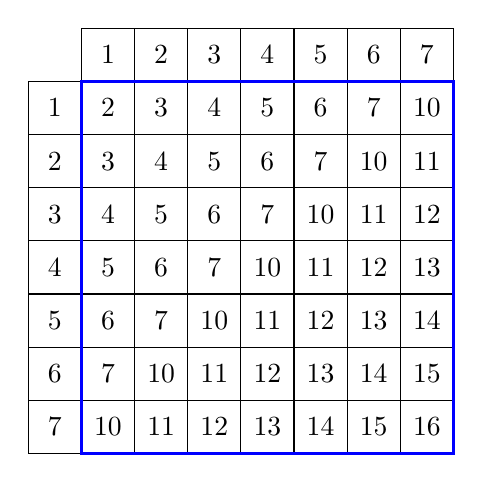
\begin{tikzpicture}[scale=0.675]
		% grid definition
		\draw (-1,0) grid (7,7);
		\draw (0,7) grid (7,8);
		\draw[line width=1pt, color=blue] (0,0) rectangle (7,7);
		
		% fill numbers
		\foreach \x in {1,2,3,...,7}
		\foreach \y in {1,2,3,...,7}
		\draw[shift={(-.5,-.5)}] (\x ,\y) node { \pgfmathoct{\number\numexpr\x+(8-\y)}\pgfmathresult\relax};
		
		% fill first row
		\foreach \x in {1,2,3,...,7}
		\draw[shift={(-.5,-.5)}] (\x , 8) node {\pgfmathoct{\x}\pgfmathresult};
		
		% fill first column
		\foreach \y in {1,2,3,...,7}
		\draw[shift={(-.5,-.5)}] (0, 8-\y) node {\pgfmathoct{\y}\pgfmathresult};
	\end{tikzpicture}
	\caption{Tavola Somma ottale}
	\label{tab:Tavolasommaottale}
\end{table}
